\documentclass[11pt]{article}
\usepackage{cite}
\usepackage{url}
\usepackage{amsthm}
\usepackage{amsmath}
\usepackage{amsfonts}
\usepackage{setspace}
\usepackage[toc,page]{appendix}
\usepackage{subcaption}
\usepackage{float}
\usepackage[pdftex]{graphicx}
\theoremstyle{plain}
\newtheorem{theorem}{Theorem}[section]
\newtheorem{corollary}[theorem]{Corollary}
\newtheorem{definition}[theorem]{Definition}
\newtheorem{lemma}[theorem]{Lemma}
\newtheorem{proposition}[theorem]{Proposition}
\newtheorem{example}[theorem]{Example}
\usepackage{listings}
\usepackage{color} %red, green, blue, yellow, cyan, magenta, black, white
\definecolor{mygreen}{RGB}{28,172,0} % color values Red, Green, Blue
\definecolor{mylilas}{RGB}{170,55,241}
\title{Homework 1.}
\author{Juan G. Garc{\'i}a}




\newcommand{\p}{\mathcal{P}}

\begin{document}
\maketitle

%Matlab's Script
\lstset{language=Matlab,%
    %basicstyle=\color{red},
    breaklines=true,%
    morekeywords={matlab2tikz},
    keywordstyle=\color{blue},%
    morekeywords=[2]{1}, keywordstyle=[2]{\color{black}},
    identifierstyle=\color{black},%
    stringstyle=\color{mylilas},
    commentstyle=\color{mygreen},%
    showstringspaces=false,%without this there will be a symbol in the places where there is a space
    numbers=left,%
    numberstyle={\tiny \color{black}},% size of the numbers
    numbersep=9pt, % this defines how far the numbers are from the text
    emph=[1]{for,end,break},emphstyle=[1]\color{red}, %some words to emphasise
    %emph=[2]{word1,word2}, emphstyle=[2]{style},    
}



%%%%%%%%%%%%%%%%%%%%%%%%%%%%%%%%%%%%%%5



\section{Fundamentals}

\subsection{Matrix Notation}
We are going to find the gradient $\nabla f$ and the Hessian $\nabla^{2} f$ of the following functions.

\subsubsection{Linear Function I}
Consider the function 

\begin{equation*}
f(w)=w^{T}a+\alpha+\sum_{j=1}^{d}w_{j}a_{j}.
\end{equation*}
Observe that this function can be written as 
\begin{equation*}
f(w)=\alpha+2\sum_{j=1}^{d}w_{j}a_{j}.
\end{equation*}
With this, the derivative with respect to the $i-th$ derivative is given by
\begin{equation*}
\frac{\partial f}{\partial w_{i}}=2a_{i},
\end{equation*}
this is the $i-th$ coordinate of the vector $2a$, hence
\begin{equation*}
\nabla f(w)=2a.
\end{equation*}
Since this function is independent of $w$ we conclude that
\begin{equation*}
\nabla^{2} f(w)=0.
\end{equation*}

\subsubsection{Linear Function II}
Now consider the function

\begin{equation*}
f(w)=a^{T}w+a^{T}Aw+w^{T}A^{T}b.
\end{equation*}
From the previous exercise we know that 
\begin{equation}\label{eqnpartI}
\nabla(a^{T}w)=a.
\end{equation}
On the other hand we have

\begin{equation*}
\frac{\partial(a^{T}Aw)}{\partial w_{i}}=\sum_{k=1}^{d}\sum_{l=1}^{d}a_{k}a_{kl}\frac{\partial w_{l}}{\partial w_{i}},
\end{equation*}
in the last equality we used the linearity of the $\frac{\partial}{\partial w_{i}}$ operator. Recalling that the coordinates $w_{i}$ 
are independent we have that $\frac{\partial w_{l}}{\partial w_{i}}=\delta_{li}$, where 
\begin{equation*}
\delta_{li}=\left\{
		\begin{array}{ll}
			1 &\mbox{if } i=j \\
			0 &\mbox{if } i\neq j
		\end{array}
	\right.
\end{equation*}
With this we conclude
\begin{equation*}
\frac{\partial(a^{T}Aw)}{\partial w_{i}}=\sum_{k=1}^{d}a_{k}a_{ki}.
\end{equation*}
This is the $i-th$ component of the vector $A^{T}a$, hence we conclude
\begin{equation}\label{eqnpartII}
\nabla(a^{T}Aw)=A^{T}a.
\end{equation}
By doing the same steps as before, it is not hard to conclude that 
\begin{equation}\label{eqnpartIII}
\nabla(w^{T}Ab)=Ab.
\end{equation}
By combining equations (\ref{eqnpartI}),(\ref{eqnpartII}) and (\ref{eqnpartIII}), we get
\begin{equation*}
\nabla f=a+A^{T}a+Ab.
\end{equation*}
Since this last expression is independent of $w$ we conclude
\begin{equation*}
\nabla^{2}f(w)=0.
\end{equation*}

\subsubsection{Cuadratic Function}
Consider the function
\begin{equation*}
f(w)=w^{T}w+w^{T}X^{T}Xw+\sum_{i=1}^{d}\sum_{j=1}^{d}w_{i}w_{j}a_{ij}.
\end{equation*}
To find the gradient, first observe that if $B$ is a $d\times d$ matrix and x is a $d\times 1$ vector then
\begin{equation*}
\nabla(\|Bx\|_{2}^{2})=2B^{T}Bx.
\end{equation*}
With this in mind we get by setting $B=I$ where $I$ is the $d\times d$ identity matrix
\begin{equation*}
\nabla(w^{T}w)=\nabla(\|w\|_{2}^{2})=2I^{T}Iw=2w.
\end{equation*}
on the other hand by setting $B=X$ we get
\begin{equation*}
\nabla(w^{T}X^{T}Xw)=\nabla(\|Xw\|_{2}^{2})=2X^{T}Xw.
\end{equation*}
Finally observe that 
\begin{equation*}
\sum_{i=1}^{d}\sum_{j=1}^{d}w_{i}w_{j}a_{ij}=w^{T}Aw.
\end{equation*}
By doing the same component-wise analysis as before we conclude 
\begin{equation*}
\nabla( w^{T}Aw)=(A+A^{T})w.
\end{equation*}
The final statement is then
\begin{equation*}
\nabla f(w)=2w+2X^{T}Xw+(A+A^{T})w=2(I+X^{T}X+\frac{A+A^{T}}{2})w.
\end{equation*}
Since the gradient of $f$ is linear w.r.t $w$ we conclude that
\begin{equation*}
\nabla^{2} f=2(I+X^{T}X+\frac{A+A^{T}}{2}).
\end{equation*}

\subsubsection{L2-regularized weighted least squares}
Observe that the first summand   can be written as
\begin{equation*}
g(w)=\sum_{i=1}^{n}v_{i}(\sum_{j=1}^{d}w_{j}x_{j}^{i}-y^{i})^{2}.
\end{equation*}
therefore by the chain rule we conclude
\begin{equation*}
\frac{\partial g(w)}{\partial w_{k}}=2\sum_{i=1}^{n}v_{i}(\sum_{j=1}^{d}w_{j}x_{j}^{i}-y^{i})\sum_{j=1}^{d}\delta_{jk}x_{j}^{i}.
\end{equation*}
That is
\begin{equation*}
\frac{\partial g(w)}{\partial w_{k}}=2\sum_{i=1}^{n}v_{i}(\sum_{j=1}^{d}w_{j}x_{j}^{i}-y^{i})x_{k}^{i}.
\end{equation*}
This is the $k-th$ component of the vector $\sum_{i=1}^{n}v_{i}(w^{T}x^{i}-y^{i})x^{i}$. On the other hand we know that
\begin{equation*}
\nabla(\|w\|_{2}^{2})=2w.
\end{equation*}
hence
\begin{equation*}
\nabla f(w)=\sum_{i=1}^{n}v_{i}(w^{T}x^{i}-y^{i})x^{i}+\lambda w.
\end{equation*}
To find the Hessian of $f$ it is convenient to remember that if $a,b,c$ are vectors then $(a^{T}b)c=(c\otimes a)b$.
Hence
\begin{equation*}
\nabla f(w)=\sum_{i=1}^{n}(x_{i}\otimes x_{i})w-\sum_{i=1}^{n}y^{i}x^{i}+\lambda w.
\end{equation*}
Since this is an affine transfomration of $w$ we conclude that
\begin{equation*}
\nabla^{2}f(w)=\sum_{i=1}^{n}x_{i}\otimes x_{i}+\lambda I.
\end{equation*}

\subsubsection{Weighted L2-regularized probit regression}



\newpage
%%%%%%%%%%%%%%%%%%%%%%%%%%%%%%%%%%%%%%%%%%%%%%%%CV%%%%%%%%%%%%%%%%%%%%%%%%%%%%%%%%%%%%%%%%%%%%%
\subsection{Cross-Validation}
\newpage








%%%%%%%%%%%%%%%%%%%%%%%%%%%%%%%%%%%%%%%%MAP estimation %%%%%%%%%%%%%%%%%%%%%%%%%%%%%%%%%%%%%%%%%%%
\subsection{MAP estimation}
\subsubsection{Laplace distribution}
We have
\begin{equation*}
y^{i}\sim\mathcal{L}(w^{T}x^{i},1),\qquad w_{j}\sim\mathcal{L}(0,\frac{1}{\lambda}).
\end{equation*}
In this case the posterior looks like (assuming independence of the variables)
\begin{equation*}
p(w|D)\propto\prod_{i=1}^{n}p(y^{i}|x^{i},w)\prod_{j=1}^{d+1}p(w_{j}).
\end{equation*}
Recalling the definition of laplaces distribution we get
\begin{equation*}
p(w|D)\propto e^{-\sum_{i=1}^{n}|y^{i}-w^{T}x_{i}|}\frac{\lambda}{2}e^{-\sum_{j=1}^{d+1}\lambda|w_{j}|}.
\end{equation*}
This means that the negative log likelihood is given by (omitting constants that don't depend on $w$)
\begin{equation*}
-\log(p(w|D))=\sum_{i=1}^{n}|y^{i}-w^{T}x_{i}|+\lambda\sum_{j=1}^{d+1} |w_{j}|.
\end{equation*}
Recalling the definition of the $L1$ norm we get that minimizing the log likelihood
is equivalent to minimize
\begin{equation*}
f(w)=\|Xw-y\|_{1}+\lambda\|w\|_{1}.
\end{equation*}


\subsubsection{Gaussians}
We now assume
\begin{equation*}
y^{i}\sim\mathcal{N}(w^{T}x^{i},\sigma_{i}^{2}),\qquad w_{j}\sim\mathcal{N}(0,\frac{1}{\lambda_{j}}).
\end{equation*}
As before we have
\begin{equation*}
p(w|D)\propto\prod_{i=1}^{n}p(y^{i}|x^{i},w)\prod_{j=1}^{d+1}p(w_{j}).
\end{equation*}
By changing products into sums in the exponenential and taking $-\log$, it is not hard
to check that 
\begin{equation*}
-\log(p(w|D))=\frac{1}{2}\sum_{i=1}^{n}\frac{(y^{i}-w^{T}x^{i})^{2}}{\sigma_{i}^{2}}+
\sum_{j=1}^{d+1}\frac{\lambda_{j}^{2}}{2}w_{j}^{2}.
\end{equation*}
If we define $\Sigma=diag(\sigma_{1},\sigma_{2},\ldots,\sigma_{n})$ and
$\Lambda=diag(\lambda_{1},\ldots,\lambda_{d+1})$ then the above equation can be written as
\begin{equation*}
-log(p(w|D)):=f(w)=\|\Sigma(Xw-y)\|_{2}^{2}+\|\Lambda w\|_{2}^{2}.
\end{equation*}

\subsubsection{Poisson Likelihood}
For this exercise we have
\begin{equation*}
y^{i}\sim\mathcal{P}(e^{w^{T}x^{i}}),\qquad w_{j}\sim\mathcal{N}(0,\frac{1}{\lambda}).
\end{equation*}
In this case by taking $-\log$ in the expression
\begin{equation*}
p(w|D)\propto\prod_{i=1}^{n}p(y^{i}|x^{i},w)\prod_{j=1}^{d+1}p(w_{j}).
\end{equation*}
and recalling that $\mathcal{P}(y;\lambda)=\frac{\lambda^{y}e^{-\lambda}}{y!}$ we get
\begin{equation*}
f(w)=\underbrace{\sum_{i=1}^{n}(e^{w^{T}x^{i}}-y^{i}w^{T}x^{i})}_{\text{Data-fitting term}}+
\frac{\lambda}{2}\|w\|_{2}^{w}.
\end{equation*}
\newpage
%%%%%%%%%%%%%%%%%%%%%%%%%%%%Convex Functions %%%%%%%%%%%%%%%%%%%%%%%%%%%%%%%%%%%%%%%%%%%%
\section{Convex Functions}

\subsection{Minimizing Strictly-Convex Quadratic Functions}

\subsubsection{Projection}
Consider
\begin{equation*}
f(w)=\frac{1}{2}\|w-v\|^{2}.
\end{equation*}
Since there are no restrictions on $w$ the obvious solution is $w=v$, then
\begin{equation*}
f(v)=0.
\end{equation*}

\subsubsection{Least Square}
For the function
\begin{equation*}
\frac{1}{2}\|Xw-y\|^{2}+\frac{1}{2}w^{T}\Lambda w.
\end{equation*}
It is convenient to remember the identities 
\begin{equation}\label{eqnnicenorm}
\nabla(\|Ax-b\|^{2})=2(A^{T}Ax-A^{T}b),
\end{equation}
and
\begin{equation*}
\nabla x^{T}Ax=(A+A^{T})w.
\end{equation*}
With this it is not hard to see that
\begin{equation*}
\nabla(f(w))=X^{T}Xw-X^{T}b+\frac{\Lambda+\Lambda^{T}}{2}w.
\end{equation*}
Setting this equation equal to zero and solving for $w$ we get
\begin{equation*}
w=\left(X^{T}X+(\Lambda+\Lambda^{T})/2\right)^{-1}X^{T}b.
\end{equation*}

\subsubsection{Weighted Least Squares Shruking to $w^{(0)}$}
In matrix notation the function of interest can be written as
\begin{equation*}
f(w)=\frac{1}{2} (Xw-y)^{T}V(Xw-y)+\frac{\lambda}{2}\|w-w^{0}\|^{2}.
\end{equation*}
Where $V$ contains the values $v_{i}\geq 0$ in the diagonal. If we define 
\begin{equation*}
\sqrt{V}=diag(\sqrt{v_{1}},\ldots,\sqrt{v_{n}}).
\end{equation*}
Then the above equation can be written as
\begin{equation*}
f(w)=\frac{1}{2}\|\sqrt{V}(Xw-y)\|^{2}+\frac{\lambda}{2}\|w-w^{0}\|^{2},
\end{equation*}
or
\begin{equation*}
f(w)=\frac{1}{2}\|\sqrt{V}Xw-\sqrt{V}y)\|^{2}+\frac{\lambda}{2}\|w-w^{0}\|^{2}.
\end{equation*}
By setting $\sqrt{V}X=A$ and $\sqrt{V}y=b$ we can use equation (\ref{eqnnicenorm}) to get
\begin{equation*}
\nabla(\frac{1}{2}\|\sqrt{V}Xw-\sqrt{V}y)\|^{2})=((\sqrt{V}X)^{T}(\sqrt{V}X)w-(\sqrt{V}X)^{T}\sqrt{V}y),
\end{equation*}
Since $\sqrt{V}$ is simmetric then $\sqrt{V}^{T}\sqrt{V}=\sqrt{V}^{2}=V$, therefore 
\begin{equation*}
\nabla(\frac{1}{2}\|\sqrt{V}Xw-\sqrt{V}y)\|^{2})=X^{T}VXw-X^{T}Vy.
\end{equation*}
On the other hand for the term $\|w-w^{0}\|^{2}$ we can use equation (\ref{eqnnicenorm}) by setting
$A=I$ and $b=w^{0}$. By doing so we get
\begin{equation*}
\nabla(\|w-w^{0}\|^{2})=2(w-w^{0}).
\end{equation*}
Hence we conclude
\begin{equation*}
\nabla f(w)=X^{T}VXw-X^{T}Vy+\lambda(w-w^{0}).
\end{equation*}

Equating to zero and solving for $w$ we obtain
\begin{equation*}
w=\left(X^ {T}VX+\lambda I\right)^{-1}\left(X^{T}Vy+\lambda w^{0}\right).
\end{equation*}

\subsection{Proving Convexity}
\subsubsection{Negative Log}
The domain of the function $-\log(aw)$ is $(0,\infty)$ which is clearly convex, on the 
other hand it is straight forward to see that 
\begin{equation*}
f''(w)=\frac{1}{w^{2}}>0,
\end{equation*}
hence $f$ is convex.

\subsubsection{Quadratic with positive semi-definite A}
for the function
\begin{equation*}
f(w)=\frac{1}{2}w^{T}Aw+b^{T}w+\gamma
\end{equation*}
its domain is all the space, hence convex domain. The gradient is given by
\begin{equation*}
\nabla f= \frac{A+A^{T}}{2}w+b,
\end{equation*}
hence its Hessian is
\begin{equation*}
\nabla^{2} f=\frac{A+A^{T}}{2}.
\end{equation*}
Since $A$ is possitive semi-definited, $A^{T}$ and $\nabla^{2} f$ are. Hence $f$ is convex.

\subsubsection{Any norm}
The domain of any norm is the whole space, hence is convex. On the other hand if $\lambda\in[0,1]$ and
$w,v\in\mathbb{R}^{d}$, then by the triangle inequality we get
\begin{equation*}
\|\lambda w+(1-\lambda)v\|_{p}\leq \lambda\|w\|_{p}+(1-\lambda)\|v\|_{p}.
\end{equation*}
which is the definition of convexity.

\subsubsection{Logistic Regression}
Finally we proved in class that the function
\begin{equation*}
f(w)=\sum_{i=1}^{n}\log(1+e^{-y_{i}w^{T}x_{i}}).
\end{equation*}
Has as Hessian
\begin{equation*}
\nabla^{2} f=X^{T}DX.
\end{equation*}
Where $D$ is a diagonal matrix with elements
\begin{equation*}
D_{ii}=sgm(y_{i}w^{T}x_{i})sgm(-y_{i}w^{T}x_{i}).
\end{equation*}
Since the sigmoind function is positive we conclude that $D$ is positive definite hence the inner product
\begin{equation*}
a^{t}Db,
\end{equation*}
induces the norm
\begin{equation*}
\|a\|_{D}:=a^{T}Da.
\end{equation*}
With this in mind if $z\in\mathbb{R}^{d}$ then
\begin{equation*}
z^{T}X^{T}DXz=\|Xz\|_{D}\geq 0.
\end{equation*}
hence $\nabla^{2} f\succeq 0$, this shows that $f$ is convex. Needless to say, to domain of $f$ is the
whole space, hence convex.
\newline
\newline
\textbf{Now we are going to prove convexity using operations that preserve convexity}

\subsubsection{regularized regression with arbitrary p-norm}
The functions
\begin{equation*}
\|Xw-y\|_{p},
\end{equation*}
and
\begin{equation*}
\lambda\|Aw\|_{q},
\end{equation*}
are composition of affine maps along with multtiplication with a positive scalar, since any norm
is convex we conclude that the function (whose domain is the whole space)  
\begin{equation*}
f(w)=\|Xw-y\|_{p}+\lambda\|Aw\|_{q},
\end{equation*}
is convex.

\subsubsection{Support Vector Regression}
constants are trivially convex, hence $0$ and $-\epsilon$ are convex,also the absolute value is convex, 
this means that 
\begin{equation*}
|y_{i}-w^{T}x_{i}|-\epsilon,
\end{equation*}
is convex. Since $\max$ and addition preserves convexity we conclude 
\begin{equation*}
\sum_{i=1}^{n} \max\{0,|w^{T}x_{i}-y_{i}|-\epsilon\},
\end{equation*}
As shown before norms are convex and since $\lambda\geq 0$ we get that 
\begin{equation*}
f(w)=\sum_{i=1}^{n} \max\{0,|w^{T}x_{i}-y_{i}|-\epsilon\}+\frac{\lambda}{2}\|w\|_{2}^{2},
\end{equation*}
is convex. Once again the domain is the whole space, which is convex.

\subsubsection{3 largest-magnitude elements}
As explained before, addition, and maximum preserves convexity and since the absolute value is convex then
\begin{equation*}
f(x)=\max_{ijk}\{|x_{i}|+|x_{j}|+|x_{k}|\},
\end{equation*}
is convex as well. In this case we assume the domain to be convex.

\newpage
\subsection{Robust Regression}

\subsubsection{robustRegression.m}
Below it is shown the script robustRegression.m
\lstinputlisting{./Q23/robustRegression.m}
Using this script on the data outliersData.mat we get the following results
\begin{figure}[H]
\centering
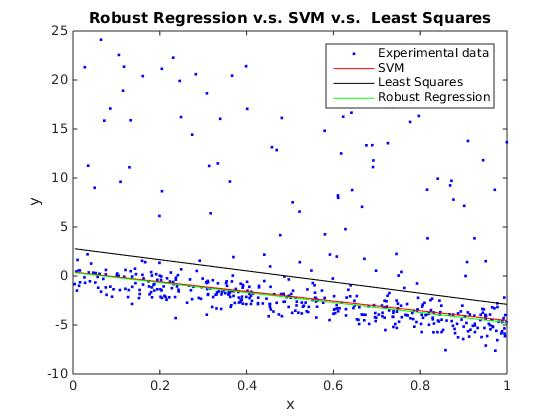
\includegraphics[scale=0.7]{./Q23/regressions}
\caption{Comparison for the robust regression with SVM and least squares.}
\label{figregressions}
\end{figure}

In this case the training error was
\begin{equation*}
\|\frac{\hat{y}-y_{test}}{500}\|_{1}=3.0666.
\end{equation*}
Now we are going to analyze how SVM behaves.


\subsubsection{SVM as a Linear Program}

For the regression problem with SVM we are going to minimize the function
\begin{equation*}
f(w)=\sum_{i=1}^{n}\max\{0,|w^{T}x_{i}-y_{i}|-\epsilon\}.
\end{equation*}

We are going to convert this into a linear program. first we define the variables $r_{i}$ to be such that
\begin{equation*}
r_{i}\geq |w^{T}x_{i}-y_{i}|-\epsilon,
\end{equation*}
and $r_{i}\geq 0$. Since $|a|=\max\{a,-a\}$ we can write the condition above as
\begin{equation*}
r_{i}\geq max\{w^{T}x_{i}-y_{i},y_{i}-w^{T}x_{i}\}-\epsilon,
\end{equation*}
or equivalently
\begin{eqnarray*}
r_{i}\geq w^{T}x_{i}-y_{i}-\epsilon,\\
r_{i}\geq y_{i}-w^{T}x_{i}-\epsilon.
\end{eqnarray*}
With this our linear problem reads as (Organizing terms to be used as inputs in Matlab)
\begin{equation*}
\min_{r\in\mathbb{R}^{n},w\in\mathbb{R}^{d}}\sum_{i=1}^{n} r_{i},
\end{equation*}
s.t.
\begin{eqnarray*}
-r_{i}\leq 0,\\
w^{T}x_{i}-r_{i}\leq y_{i}+\epsilon, \\
-w^{T}x_{i}-r_{i}\leq -y_{i}+\epsilon.
\end{eqnarray*}


\subsubsection{SVM Regression}
Now we do a regression using the script svRegression.m shown below

\lstinputlisting{./Q23/svRegression.m}

The regression obtained for $\epsilon=1$ is shown in Figure \ref{figregressions}. For this case 
the training error was
\begin{equation*}
\|\frac{\hat{y}-y_{test}}{500}\|_{1}=3.0746.
\end{equation*}
Using SVM with $\epsilon=1$ was slightly less accurate than robust regression.





\end{document}
